\chapter{Teorie výpočtu}
\label{kap:teorie}
	V této kapitole bych rád čtenáře seznámil s teoretickými poznatky, ze kterých jsem při mém návrhu vycházel. Celá tato kapitola \ref{kap:teorie} je parafrázováním knihy \cite{Rychetnik:Motory} doplněné o některé mé postřehy a poznámky. Kapitola je rozdělena na dvě části – v první se zabývám teoretickou účinností větrných motorů. V druhé části popisuji funkci horizontální vztlakové turbíny a uvádím dva způsoby výpočtu.
	
	\section{Teoretická účinnost větrných turbín}\label{ucinnost}
	Jak jsem již zmínil v kapitole \ref{sec:typy_turbin}, základy funkce vztlakových turbín popsal Albert Betz. Ten odvodil maximální teoretickou účinnost větrných motorů. Na jeho počest je nazývána Betzova.
	
	Je několik různých způsobů výpočtů maximální účinnosti. Některé dávají vyšší a některé nižší hodnoty (např. maximální účinnost podle Sabinina je 68,7~\% \cite{Rychetnik:Motory}). Běžně se však v literatuře uvažuje právě Betzova účinnost. Tato účinnost je pouze teoretická. Skutečná účinnost je vždy značně nižší (aby se turbína mohla přiblížit ideální, nesměla by proudu vzduchu za ní udělovat rotační složku).
	V této kapitole bych rád ukázal, jak lze Betzovu účinnost odvodit. Odvození vychází z~obrázku~\ref{obr.rotor}:
	\begin{figure}[H]
		%\begin{center}
		\centering
			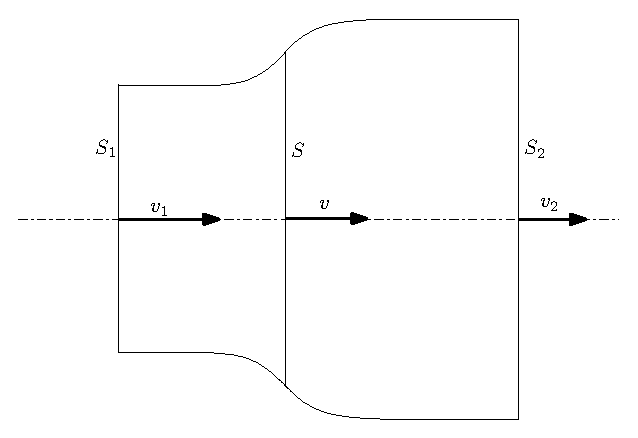
\includegraphics[]{obrazky/rotor}
	          %\input{obrazky/rotor2.ipe}
		\caption{Princip větrné turbíny. Proud vzduchu (v ploše $S_1$ s rychlostí $v_1$) vstupuje do roviny turbíny $S$. Zde je zpomalen a za rotorem vystupuje v ploše $S_2$ s rychlostí $v_2$. Inspirováno \cite{Rychetnik:Motory}.}
		\label{obr.rotor}
	    %\end{center}
	  \end{figure}
	
	Tento nákres znázorňuje proud vzduchu procházející rotorem. Za předpokladu, že se tento proud nemísí s okolním vzduchem, je soustava izolovaná a platí zde rovnice kontinuity \eqref{rov:1}\cite{Rychetnik:Motory}:
	
	\begin{equation}
		S_1 v_1 = Sv = S_2 v_2\label{rov:1}
	\end{equation}
	Poté lze za zákona zachování hybnosti odvodit axiální sílu $F_a$ působící na rotor \eqref{rov:2}\cite{Rychetnik:Motory}:
	\begin{eqnarray}
		\label{rov:2}
		\Delta p = p_1 - p_2 \nonumber \\
		F\Delta t=mv_1 - mv_2 \nonumber \\
		F\Delta t = \rho Sv\Delta t(v_1 - v_2) \nonumber \\
		F_a = \rho Sv(v_1 - v_2)
	\end{eqnarray}
	Z axiální síly $F_a$ lze spočítat i výkon turbíny \eqref{rov:3}\cite{Rychetnik:Motory}:
	\begin{equation}
		\label{rov:3}
		P = F_a v = \rho Sv^2 (v_1 - v_2)
	\end{equation}
	Výkon turbíny lze také spočítat i pomocí změny kinetické energie proudu vzduchu \eqref{rov:4}\cite{Rychetnik:Motory}:
	\begin{equation}
			\label{rov:4}
			P = \frac{\Delta E_k}{\Delta t} = \frac{1}{2} \rho Sv(v_1^2 - v_2^2)
	\end{equation}
	Porovnáním různě vyjádřeného výkonu z rovnice \ref{rov:3} a \ref{rov:4} vyplývá, že rychlost v rovině rotoru je aritmetickým průměrem rychlosti před a za rotorem \eqref{rov:5}\cite{Rychetnik:Motory}:
	\begin{equation}
			\label{rov:5}
			P_p = P_{E_k} \Rightarrow v=\frac{v_1 + v_2}{2}
	\end{equation}
	Díky tomuto poznatku lze vyjádřit axiální sílu $F_a$ i výkon $P$ pouze v závislosti na rychlosti proudu větru před a za rotorem\eqref{rov:6}\cite{Rychetnik:Motory}:
	\begin{eqnarray}
		\label{rov:6}
		F_a = \frac{1}{2}\rho S(v_1^2 - v_2^2) \nonumber \\
		P=\frac{1}{4}\rho S(v_1^2 - v_2^2)(v_1 + v_2)
	\end{eqnarray}
	Účinnost můžeme vyjádřit jako poměr výkonu turbíny a výkonu proudu vzduchu vstupujícího do turbíny vzduchu\eqref{rov:7}\cite{Rychetnik:Motory}. Výkon proudu vzduchu lze určit pomocí kinetické energie tohoto proudu.
	\begin{equation}
		\label{rov:7}
		\eta = \frac{\frac{1}{4}\rho S(v_1^2 - v_2^2)(v_1 + v_2)}{\frac{1}{2}\rho Sv_1^3}=\frac{(v_1^2 - v_2^2)(v_1 + v_2)}{2v_1^3}
	\end{equation}
	Pokud vyjádříme poměr rychlostí proudu vzduchu před a za rotorem následovně\eqref{rov:8}\cite{Rychetnik:Motory}:
	\begin{equation}
		\label{rov:8}
		k= \frac{v_2}{v_1}
	\end{equation}
	Lze rovnici \eqref{rov:7} zjednodušit na tvar \eqref{rov:9}
	\begin{equation}
		\label{rov:9}
		\eta = \frac{(k+1)(1-k^2)}{2}
	\end{equation}
	Derivací tohoto výrazu můžeme zjistit jeho maximum\eqref{rov:10}:
	\begin{eqnarray}					\label{rov:10}
		\frac{\mathrm{d}}{\mathrm{d}k}(\frac{(k+1)(1-k^2)}{2})=\frac{-3k^2}{2}-k+\frac{1}{2} \nonumber \\
		\frac{-3k^2}{2}-k+\frac{1}{2}=0 \Rightarrow k=\{-1;\frac{1}{3}\}
	\end{eqnarray}
	Výraz \ref{rov:10} má maximální hodnotu na intervalu $<0;1>$ (jiné hodnoty poměru rychlostí nedávají smysl) pro $k=\frac{1}{3}$. Při tomto poměru rychlostí vychází $\eta =\frac{16}{27}\doteq 59~\%$, což je hledaná Betzova teoretická účinnost. Průběh účinnosti v závisloti na poměru rychlostí lze vidět na grafu \ref{graf.ucinnost}.
	\begin{figure}[H]
		%\begin{center}
		\centering
			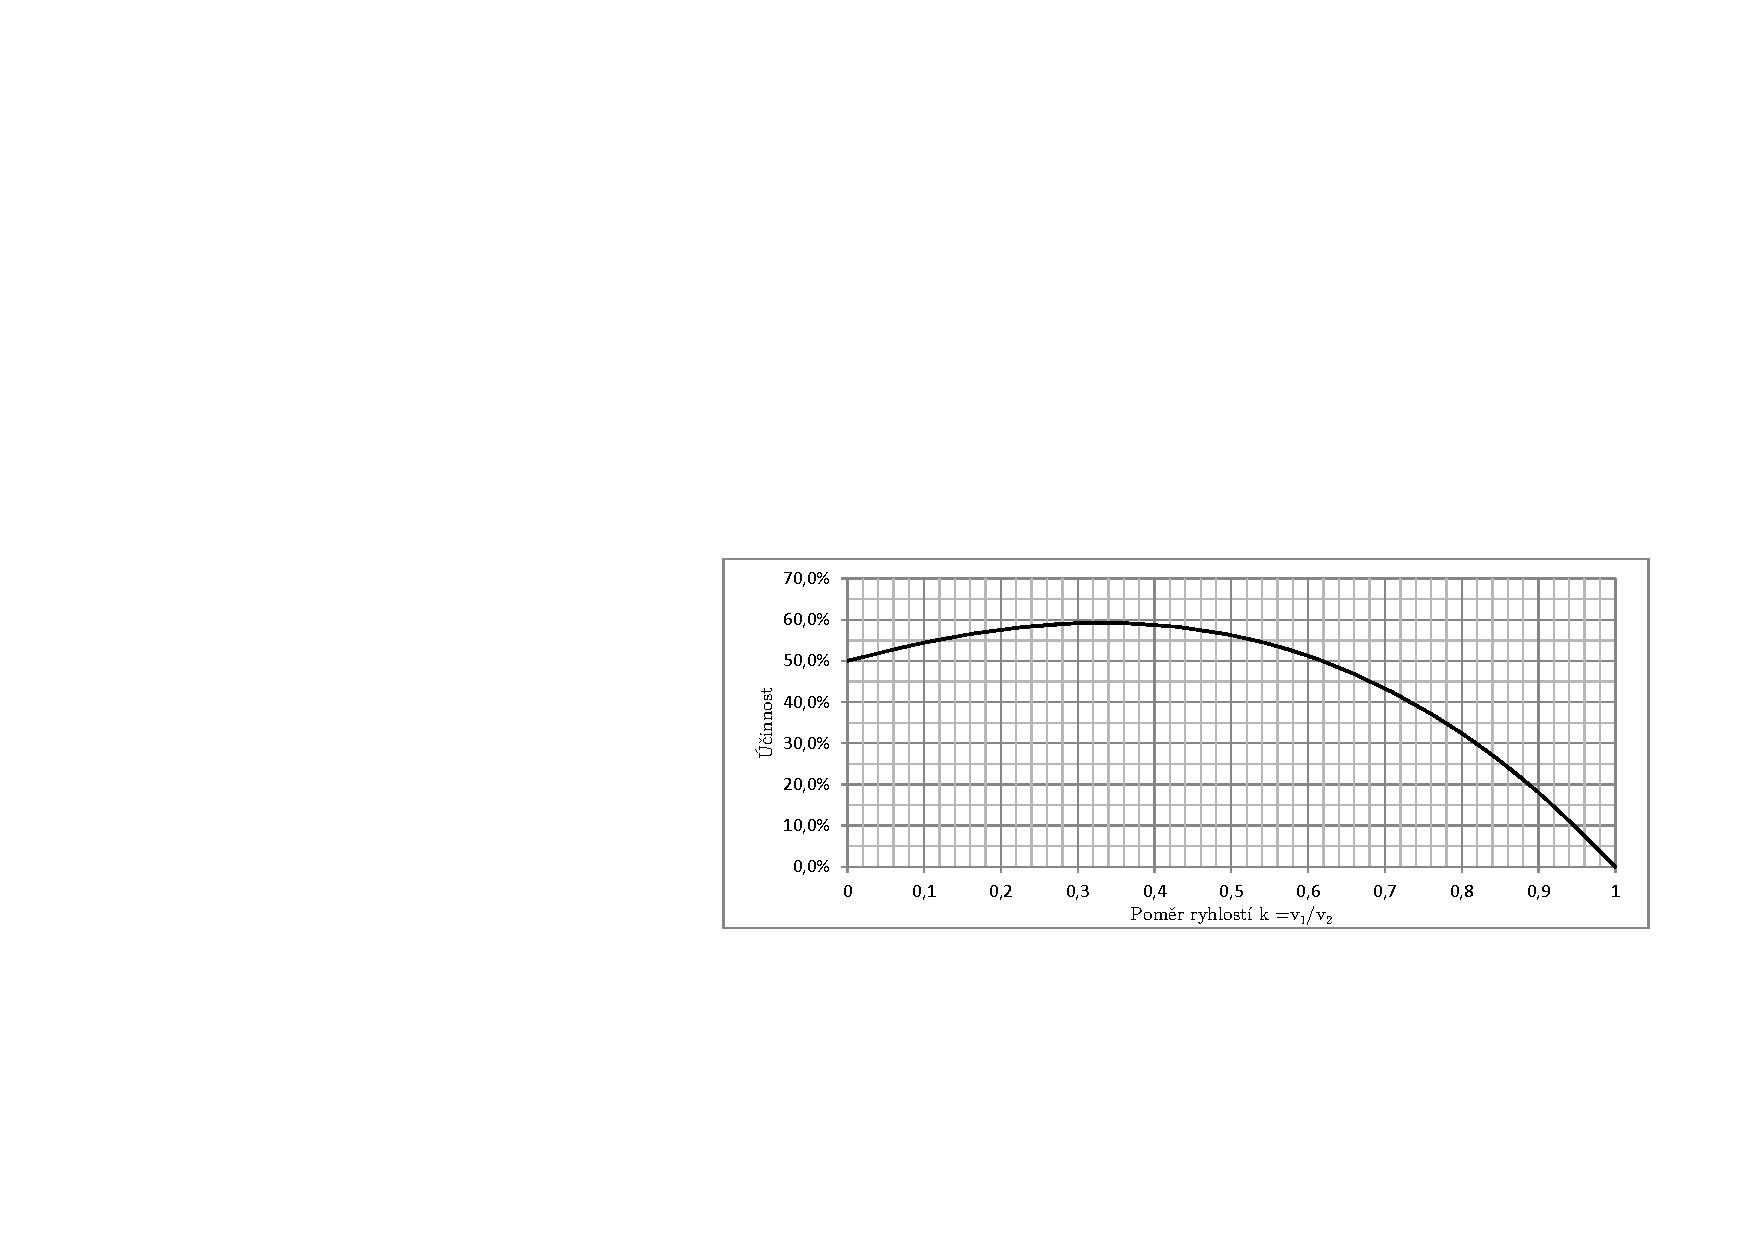
\includegraphics[]{obrazky/grafy/ucinnost}
	          %\input{obrazky/rotor2.ipe}
		\caption{Průběh Betzovy účinnosti pro jednotlivé poměry $v_1/v_2$}
		\label{graf.ucinnost}
	    %\end{center}
	  \end{figure}
	  
	\section {Aerodynamika horizontální vztlakové turbíny}
	V této kapitole shrnuji veškeré důležité teoretické poznatky pro výpočet větrné turbíny. Tyto poznatky jsou poté použity k výpočtu parametrů turbíny v kapitole \ref{chap:praxe}.
	
	Tuto kapitolu jsem rozdělil na tři části. V první části (kapitola \ref{kap:zakladprinc}) jsou vysvětleny základní principy a pojmy ohledně aerodynamických profilů – základního stavebního prvku vztlakových turbín.
	
	Druhá část (kapitola \ref{kap:funkce1}) vysvětluje funkci turbíny a odvozuje základní výpočet. Na tuto kapitolu navazuje kapitola \ref{kap:funkce2}, která tento výpočet rozšiřuje o vírovou teorii.
	
	\subsection{Základní princip, aerodynamický profil}\label{kap:zakladprinc}
	Jak jsem zmínil v předchozích kapitolách, základním principem vztlakových turbín je síla vznikající na rotorovém listu při obtékání vzduchem. Tato síla vzniká díky tvarování listu – podobně jako na křídle letadla. List má v průřezu tvar aerodynamického profilu.
	
	Aerodynamický profil lze nejlépe charakterizovat pomocí obrázku \ref{obr.profil}:
	
	\begin{figure}[H]
		\centering
		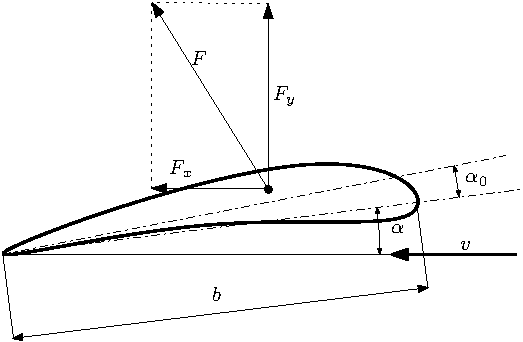
\includegraphics[]{obrazky/profil.pdf}
		\caption{Charakteristika aerodynamického profilu. Inspirováno \cite{Rychetnik:Motory}}
		\label{obr.profil}
	\end{figure}
	
	Profily mají různý tvar; zpravidla jsou však na své náběžné hraně zakulacené a směrem k~odtokové hraně se sbíhají do ostrého konce. Spojnice odtokové hrany s~náběžnou se nazývá tětiva profilu. Zpravidla se značí~$b$. Úhel, který svírá tětiva profilu se směrem pohybu proudu vzduchu (rychlost je zde označena jako $v$), se nazývá úhel náběhu. Běžně se označuje $\alpha$. Často se úhlem $\alpha$ automaticky myslí optimální úhel náběhu, při kterém profil vykazuje nejlepší vlastnosti (poměr sil $F_y$ a $F_x$ je největší). Na obrázku je také vyznačen úhel $\alpha _0$ – úhel nulového vztlaku. Při tomto úhlu náběhu nevzniká na profilu žádná vztlaková síla\cite{Rychetnik:Motory}.
	
	Při obtékání profilu proudem vzduchu vzniká síla $F$. Její velikost a směr jsou závislé na úhlu~$\alpha$. Síla zde vzniká díky vyšší rychlosti obtékajícího vzduchu na vztlakové (na nákresu se jedná o horní stranu) než na podtlakové (spodní) straně. Podle Bernoulliho rovnice klesá v~rychleji se pohybujícím proudu vzduchu statický tlak. Tento podtlak vyvolává vztlakovou sílu\cite{Rychetnik:Motory}.
	
	Pro další úvahy je vhodné rozdělit sílu $F$ na dvě navzájem kolmé složky – $F_x$ a $F_y$. Sílu $F_y$, která je kolmá na směr pohybu proudu vzduchu, nazýváme vztlaková (anglicky označována jako lift force). Sílu $F_x$ nazýváme odporovou (anglicky drag force). Tato síla působí proti směru pohybu profilu a je nežádoucí – snižuje účinnost rotoru\cite{Rychetnik:Motory}\cite{ve:ve}.
	
	Velikost těchto sil je možno spočítat pomocí součinitele vztlaku $c_y$ (v anglické literatuře označován jako $c_L$ – lift coefficient) a součinitele odporu $c_x$ (ang. $c_d$, drag coefficient). Tyto součinitelé jsou vždy platní pouze pro určitý úhel náběhu a Reynoldsovo číslo (viz dále). Dají se zjistit experimentálně, případně pomocí CFD simulace. Na základě těchto součinitelů lze síly $F_x$ a $F_y$ spočítat následovně \eqref{rov:11}\cite{Rychetnik:Motory}:
	
	\begin{eqnarray}
			\label{rov:11}
			F_x \frac{1}{2}\rho c_x Sv^2 \nonumber \\
			F_y \frac{1}{2}\rho c_y Sv^2
	\end{eqnarray}
	Kde $\rho$ označuje hustotu vzduchu, $v$ rychlost proudu vzduchu a $S$ plochu listu. V dalších kapitolách bude často uvažována nekonečně malá část rotorového listu a za $S$ se bude dosazovat $dS$, které lze definovat následovně\eqref{rov:12}\cite{Rychetnik:Motory}: 
	
		\begin{equation}
				\label{rov:12}
				S=b\;\mathrm{d}r
		\end{equation}
	Kde $\mathrm{d}r$ je nekonečně malá vzdálenost mezi 2 poloměry $r_1$ a $r_2$ na rotorovém listu a $b$ je délka tětivy.
	
	Na grafech \ref{graf:zavislost1} a \ref{graf:zavislost2} je znázorněn průběh součinitelů vztlaku a odporu v závislosti na úhlu náběhu pro profil SG6043 (při Reynoldsově čísle $10^5$).
	
	\begin{figure}[H]
	\centering
	\subfigure[Závislost součinitele vztlaku na úhlu náběhu. ]{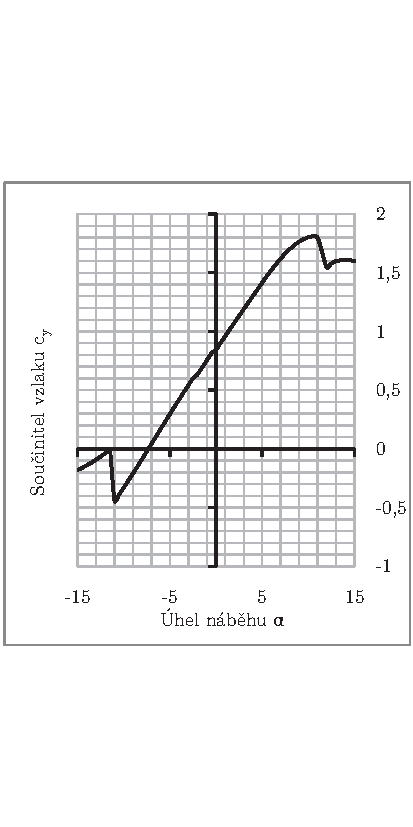
\includegraphics[]{obrazky/grafy/odvozeni3p}\label{graf:zavislost1}}~
	\subfigure[Závislost součinitele odporu na úhlu náběhu. ]{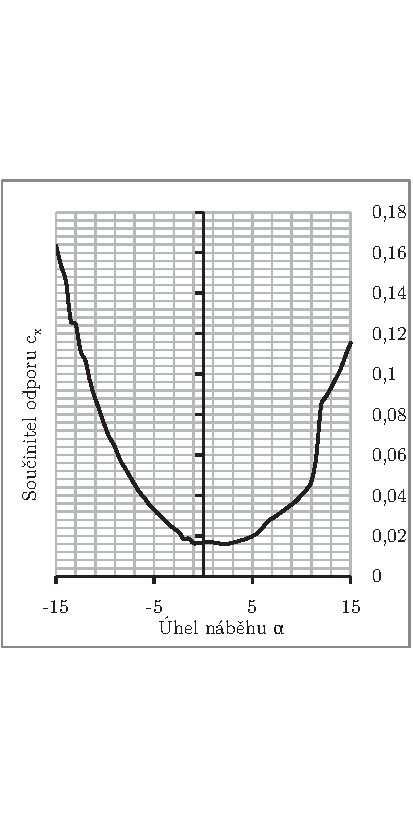
\includegraphics[]{obrazky/grafy/odvozeni2p}\label{graf:zavislost2}}
	\caption{Závislosti součinitelů $c_x$ a $c_y$ u profilu SG6043 při $Re=10^5$. Data převzata z \cite{profil}}
	\end{figure}
	
	Jak jsem zmínil výše, aerodynamické vlastnosti profilu nejsou vždy stejné. Pro charakteristiku podmínek, při kterých byly naměřeny dané hodnoty, se používá Reynoldsovo číslo $Re$. Jedná se o bezrozměrnou veličinu popisující proudění. Reynoldsovo číslo je definováno následovně\eqref{rov:13}\cite{Rychetnik:Motory}:
	\begin{equation}
					\label{rov:13}
					Re=\frac{vl}{\nu}
	\end{equation}
	Kde ve vztahu \eqref{rov:13} $v$ je rychlost obtékání profilu, $l$ je délka tětivy a $\nu$ je kinematická viskozita vzduchu.
	
	Reynoldsovo číslo se pohybuje pro malé rotory (do 10~m) v rozmezí $10^5$–$10^7$\cite{ve:ve}. Ze vzorce je patrné, že Reynoldsvo číslo je pouze orientační údaj – ve vzorci vystupuje rychlost obtékání a~délka tětivy. Obě tyto veličiny se u listů větrné turbíny mění v závislosti na vzdálenosti od osy otáčení. Proto se také často počítá se zaokrouhlenou hodnotou kinematické viskozity vzduchu $1,5\cdot 10^{-6}\;m\cdot s^{-2}$\cite{Rychetnik:Motory}.
	
	\subsection{Funkce horizontální vztalkové turbíny}\label{kap:funkce1}
	Cílem této kapitoly je objasnit, jaký tvar (úhel náběhu a délku tětivy) by rotorový list měl mít, aby dosahoval co nejlepších vlastností.
	
	Na otáčející se turbíně se nachází rotorový list v~situaci na obrázku \ref{obr.profilprostor}).
	
	\begin{figure}[H]
		\centering
		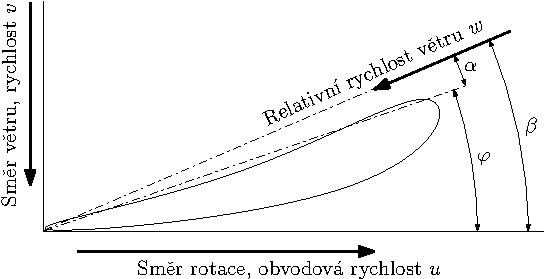
\includegraphics[]{obrazky/profilnavrtuli}
		\caption{Rotorový list na otáčející se turbíně. Inspirováno \cite{Rychetnik:Motory}.}
		\label{obr.profilprostor}
	\end{figure}
	Obrázek \ref{obr.profilprostor} zobrazuje část (řez) rotorového listu na poloměru $r$. Celý list se otáčí úhlovou rychlostí $\omega$, prvek na poloměru $r$ má pak tedy obvodovou rychlost $u$ \eqref{rov:14}\cite{Rychetnik:Motory}:
	\begin{equation}
		\label{rov:14}
		u=\omega r=\frac{\pi n}{30}r
	\end{equation}
	Kde $n$ jsou otáčky za minutu, které jsou zde uvedeny, jelikož jsou pro představu názornější než úhlová rychlost. Rovnoběžně s~osou otáčení fouká vítr rychlostí $v$. Je důležité si všimnout orientace profilu listu – tlaková strana je nastavena proti směru větru. Je tedy opačně orientován než u běžných leteckých vrtulí. U leteckých vrtulí má list opačnou funkci – místo zpomalování proud vzduchu jej urychluje.
	
	Vektorovým součtem obvodové rychlosti $u$ a rychlosti větru $v$ získáváme relativní rychlost větru $w$. Platí tedy \eqref{rov:15}\cite{Rychetnik:Motory}.
	\begin{equation}
		\label{rov:15}
		w=\sqrt{u^2 + v^2}
	\end{equation}
	Rychlostí $w$ (a v jejím směru) je rotorový list ofukován. Na obrázku je vyznačen úhel $\beta$, který rychlost $w$ svírá s~osou otáčení. Z~obrázku je tedy patrný vztah \eqref{rov:16}\cite{Rychetnik:Motory}:
	\begin{equation}
		\label{rov:16}
		\tan{\beta}=\frac{v}{u}
	\end{equation}
	Z rovnice \eqref{rov:16} vyplývá důležitý poznatek – jelikož je rychlost v konstantní a obvodová rychlost u závisí na poloměru $r$, nemá rotorový list po celé své délce stejný úhel náběhu. Obdobně se dá předpokládat, že ani délka tětivy $b$ nebude po celé délce listu konstantní. Proto musí být veškeré úvahy prováděny na (nekonečně) malém úseku mezi poloměrem $r$ a $r + \mathrm{d}r$.
	
	Úhel $\alpha$, který svírá tětiva profilu s~relativní rychlostí proudu vzduchu, zde značí optimální úhel náběhu – poměr součinitelů $c_y/c_x$ je největší možný pro daný profil.
	
	Na rotorovém listu při obtékání vzduchem vzniká vztlaková síla. Tu můžeme rozložit podle obrázku \ref{obr.profilsil}.
	\begin{figure}[h]
		\centering
		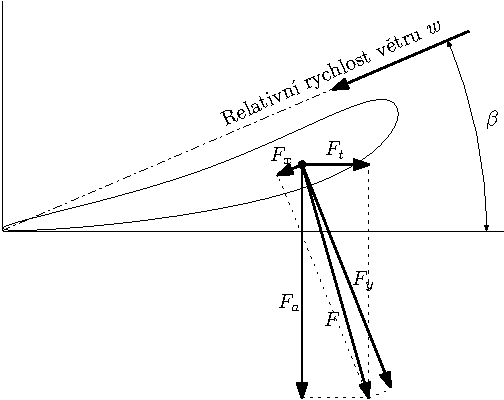
\includegraphics[]{obrazky/sily}
		\caption{Rozklad sil na rotorovém listu. Inspirováno \cite{Rychetnik:Motory}.}
		\label{obr.profilsil}
	\end{figure}
	Síly $F_x$ a $F_y$ lze spočítat z rovnice \ref{rov:11}. Jejich výslednice lze rozložit na 2 složky – sílu $F_t$, která otáčí rotorem, a sílu $F_a$, která působí na stožár a na užitečném výkonu turbíny se nepodílí. Síla $F_t$, respektive její element $\mathrm{d}F_t$ na prvku $r$, vyvolává elementární moment síly dle \eqref{rov:17}\cite{Rychetnik:Motory}.
	\begin{equation}
		\label{rov:17}
		\mathrm{d}M=\mathrm{d}F_t r
	\end{equation}
	Jelikož se v dalších výrazech vyskytuje úhel $\beta$, je vhodné vyjádřit $w$ také pomocí úhlu $\beta$ \eqref{rov:18}\cite{Rychetnik:Motory}:
	\begin{eqnarray}
				\label{rov:18}
			u=v \cot\beta \nonumber \\
			w^2 = 1 + cotg^2 \beta
	\end{eqnarray}
	Poté lze vyjádřit sílu v axiálním směru ve tvaru \eqref{rov:19}\cite{Rychetnik:Motory}.
	\begin{equation}
		\label{rov:19}
		\mathrm{d}F_a=\frac{1}{2}v^2\rho\;\mathrm{d}S(1+cotg^2 \beta)(c_y \cos \beta + c_x \sin \beta)
	\end{equation}
	Kde $(c_y \cos\beta+c_x \sin \beta)$ vychází z obrázku \ref{obr.odvozeni1}.
	\begin{figure}[H]
		\centering
		\subfigure[Zde lze vidět, že síla $F_a$ je složena z~přilehlé odvěsny přepony velkého trojúhelníku s~úhlem $\beta$ a protihlehlé odvěsny malého trojúhelníku s~úhlem~$\beta$ ]{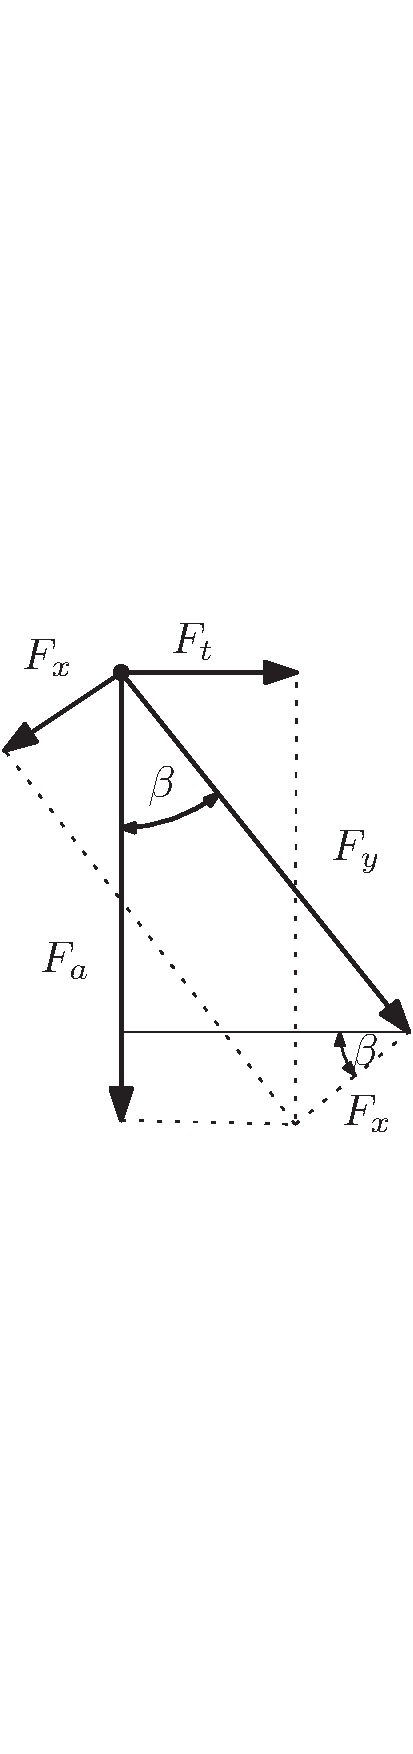
\includegraphics[]{obrazky/odvozeniplusp}\label{obr.odvozeni1}}~
		\subfigure[Zde lze vidět, že síla $F_t$ je rovna protilehlé odvěsně velkého trujúhelníku s~úhlem $\beta$ mínus přilehlá odvěsna malého trojúhelníku s~úhlem~$\beta$]{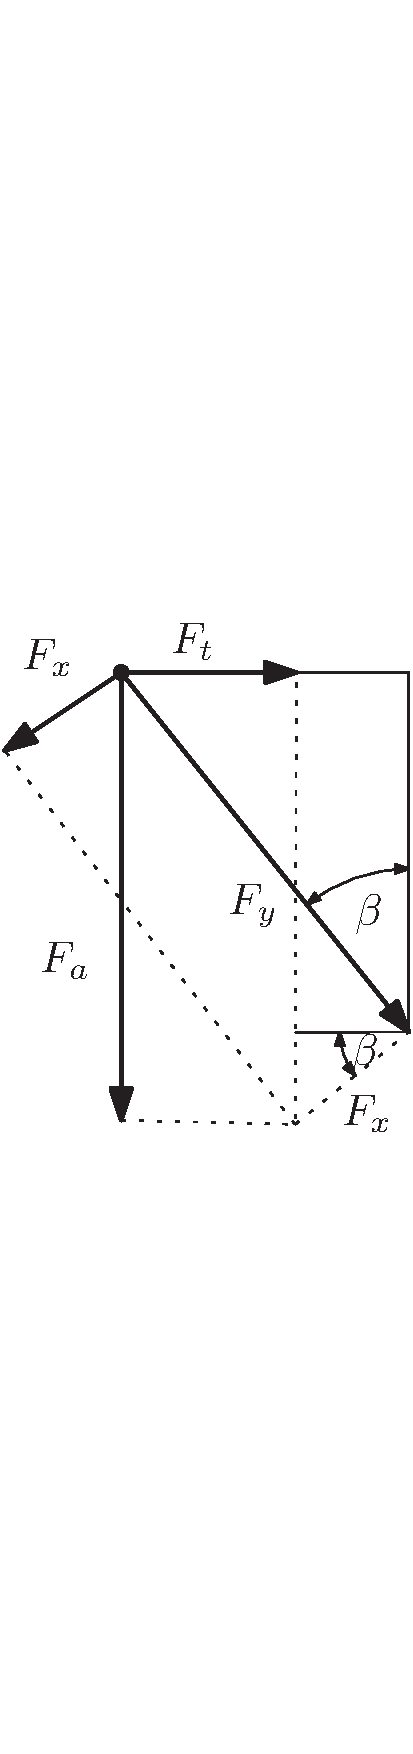
\includegraphics[]{obrazky/odvozeniminusp}\label{obr.odvozeni2}}
		\caption{Odvození vztahů pro síly na profilu}
	\end{figure}
	Obdobně lze vyjádřit i element síly $F_t$ \eqref{rov:20}\cite{Rychetnik:Motory}.
	\begin{equation}
			\label{rov:20}
			\mathrm{d}F_t=\frac{1}{2}v^2\rho\;\mathrm{d}S(1+cotg^2 \beta)(c_y \sin \beta - c_x \cos \beta)
	\end{equation}
	V knize \cite{Rychetnik:Motory} se ve výrazu \eqref{rov:20} nachází chyba (překlep), kdy je v poslední závorce znaménko plus místo mínus. Důkaz znaménka mínus vyplývá z obrázku \ref{obr.odvozeni2}.
	
	Z výše vyjádřené síly $F_t$ lze určit elementární moment a elementární užitečný výkon vznikající na daném prvku rotoru \eqref{rov:21}\cite{Rychetnik:Motory}.
	\begin{eqnarray}
		\label{rov:21}
		\mathrm{d}M=\frac{1}{2}v^2\rho \; \mathrm{d}Sr(1+cotg^2 \beta) (c_y\sin\beta - c_x\cos \beta)\nonumber \\
		\mathrm{d}P_u=\mathrm{d}M\omega=\mathrm{d}M\frac{u}{r}=\mathrm{d}M\frac{v \cot\beta}{r}\nonumber \\
		\mathrm{d}P_u=\frac{1}{2}v^3\rho\;\mathrm{d}S(1+cotg^2 \beta)(c_y\sin \beta-c_x\cos\beta)\cot\beta
	\end{eqnarray}
	Tímto byly shrnuty veškeré základní poznatky, které je nutno o vztlakové horizontální turbíně vědět. Zbývá už jen z~těchto poznatků vyjádřit, jak má co nejideálnější turbína vypadat.
	
	Základním parametrem větrné turbíny je již dříve zmíněná rychloběžnost. Zpravidla se značí~$\lambda$ (někdy se lze setkat i s~označením $\lambda_0$). Jedná se o bezrozměrnou veličinu, která popisuje poměr obvodové rychlosti turbíny $u_R$ vůči rychlosti větru před turbínou $v_1$\eqref{rov:22}\cite{Rychetnik:Motory}.
	\begin{equation}
			\label{rov:22}
			\lambda = \frac{u_R}{v_1}
	\end{equation}
	Tento parametr turbíny se zpravidla volí (odvisí od něj otáčky rotoru), je však omezen daným typem turbíny. Například rotor Savonius je schopný efektivně pracovat při rychloběžnosti 0,85–1,8, \uv{americké kolo} 1,1–2, třílistá horizontální turbína 2–6, dvoulistá 6–10. Třílistý rotor Darrieus 4,6–6,8 a jednolistý 6–10. Tyto údaje byly převzaty z~\cite{Rychetnik:Motory} a~\cite{ve:ve}. Z~předchozích poznatků vyplývá, že ideální rotor má konstantní rychloběžnost a tudíž je neregulovatelný. Jakoukoliv regulaci otáček je možné provést pouze za cenu snížení účinnosti.
	
	Můžeme také definovat rychloběžnost pro prvek na listu ve vzdálenosti $r$ od středu \eqref{rov:23}\cite{Rychetnik:Motory}.
	\begin{equation}
		\label{rov:23}
		\lambda_r = \frac{u_r}{v_1}=\frac{r}{R}\lambda
	\end{equation}
	V kapitole \ref{ucinnost} vyplynulo z Betzovi účinnosti, že rotor má maximální účinnost právě tehdy, platí-li \eqref{rov:24}.	
	\begin{equation}
			\label{rov:24}
			v_2 = \frac{1}{3}v_1
	\end{equation}
	Z rovnice \eqref{rov:5} v kapitole \ref{ucinnost} vyplývá, že rychlost v rovině rotoru $v$ je rovna \eqref{rov:25}\cite{Rychetnik:Motory}.
	\begin{equation}
		\label{rov:25}
		v = \frac{v_1+v_2}{2}=\frac{v_1+\frac{1}{3}v_1}{2}=\frac{2}{3}v_1
	\end{equation}
	Díky vyjádření z~rovnice \eqref{rov:25} lze dosazením do rovnice \eqref{rov:16} spočítat~$\beta$ pro jednotlivé prvky listu ve vzdálenosti~$r$ od středu rotoru\eqref{rov:26} – tedy jednu ze dvou charakteristik tvaru listu (druhou je délka tětivy)\cite{Rychetnik:Motory}.
	\begin{eqnarray}
		\label{rov:26}
		\tan\beta=\frac{v}{u_r}=\frac{\frac{2}{3}v_1}{\lambda_r v_1}=\frac{2}{\frac{3r\lambda}{R}} \nonumber \\
		\beta = \arctan(\frac{2R}{3r\lambda})
	\end{eqnarray}
	K tomuto vyjádření je nutné připomenout obrázek \ref{obr.profilprostor}. Z~něj je patrné, že úhel $\beta$ není odchylkou tětivy profilu od roviny rotoru. Odchylku tětivy profily je úhel $\varphi$, který lze určit dle \eqref{rov:27}.
	\begin{equation}
		\label{rov:27}
		\varphi = \beta - \alpha
	\end{equation}
	Kde $\alpha$ je optimální úhel náběhu daného aerodynamického profilu.
	
	Délku tětivy lze spočítat z předpokladu, který vyplývá z Betzovy účinnosti – proud vzduchu musí být turbínou zpomalen na $\frac{1}{3}$  své původní rychlosti. Proud vzduchu vyvolává na rotoru axiální sílu. Axiální sílu působící na jeden element rotoru lze změnou hybnosti vyjádřit dle \eqref{rov:28}\cite{Rychetnik:Motory}.
	\begin{eqnarray}
		\label{rov:28}
		\mathrm{d}F_a=\rho\; \mathrm{d}V(v_1 - v_2) \nonumber \\
		\mathrm{d}V=2\pi r \; \mathrm{d}r\frac{v_1+v_2}{2} \nonumber \\
		\mathrm{d}F_a=2\pi\rho r\; \mathrm{d}r\frac{v_1+v_2}{2}(v_1-v_2)
	\end{eqnarray}
	Axiální sílu lze však vyjádřit i pomocí aerodynamických sil (jak je popsáno v rovnici \eqref{rov:19}). Kniha \cite{Rychetnik:Motory} tento výpočet dle mě zbytečně zjednodušuje – zanedbává vliv odporové síly vznikající na profilu listu. Já jej však budu nadále uvažovat. Rovnice \eqref{rov:19} však představuje sílu působící pouze na jeden list; celková síla axiální síla je \eqref{rov:29}:
	\begin{equation}
			\label{rov:29}
			\mathrm{d}F_a=\frac{1}{2}v^2z\rho\;\mathrm{d}S(1+cotg^2 \beta)(c_y \cos \beta + c_x \sin \beta)
	\end{equation}
	Kde $z$ je počet listů rotoru.
	
	Porovnáním dvou vyjádření axiální síly a dosazením vztahů \eqref{rov:28} a \eqref{rov:29} lze získat vztah \eqref{rov:30} vyjadřující délku tětivy $b$ pro element listu na poloměru $r$.
	
	\begin{eqnarray}
		\label{rov:30}
		2\pi\rho r\; \mathrm{d}r\frac{v_1+v_2}{2}(v_1-v_2)=\frac{1}{2}\left( \frac{v_1 + v_2}{2} \right)^{2} z\rho b\;\mathrm{d}r(1+cotg^2 \beta)(c_y \cos \beta + c_x \sin \beta) \nonumber \\
		2\pi r(v_1-v_2)=\frac{1}{2} zb(1+cotg^2 \beta)(c_y \cos \beta + c_x \sin \beta)\left( \frac{v_1 + v_2}{2} \right) \nonumber \\
		2\pi r\frac{2}{3}v_1=\frac{1}{2} zb(1+cotg^2 \beta)(c_y \cos \beta + c_x \sin \beta )\frac{2}{3}v_1 \nonumber \\
		b=\frac{4\pi r}{z(1+cotg^2 \beta)(c_y \cos \beta + c_x \sin \beta )}
	\end{eqnarray}
	Toto vyjádření není v ideální podobě (bylo by vhodné ještě vyjádřit funkce úhlu $\beta$ pomocí poloměru a rychloběžnosti), ale i přesto poskytuje jasnou představu o délce tětivy na listu.
	
	Na grafech \ref{graf.delka1} a \ref{graf.nabeh1} lze najít průběh délky tětivy a úhlu odchylky tětivy od rotoru na prvním prototypu větrné turbíny. Je zde zahrnuto i porovnání výpočtu uvažujícího odporovou sílu a výpočtu, který ji neuvažuje.
	
	\begin{figure}[H]
			%\begin{center}
			\centering
				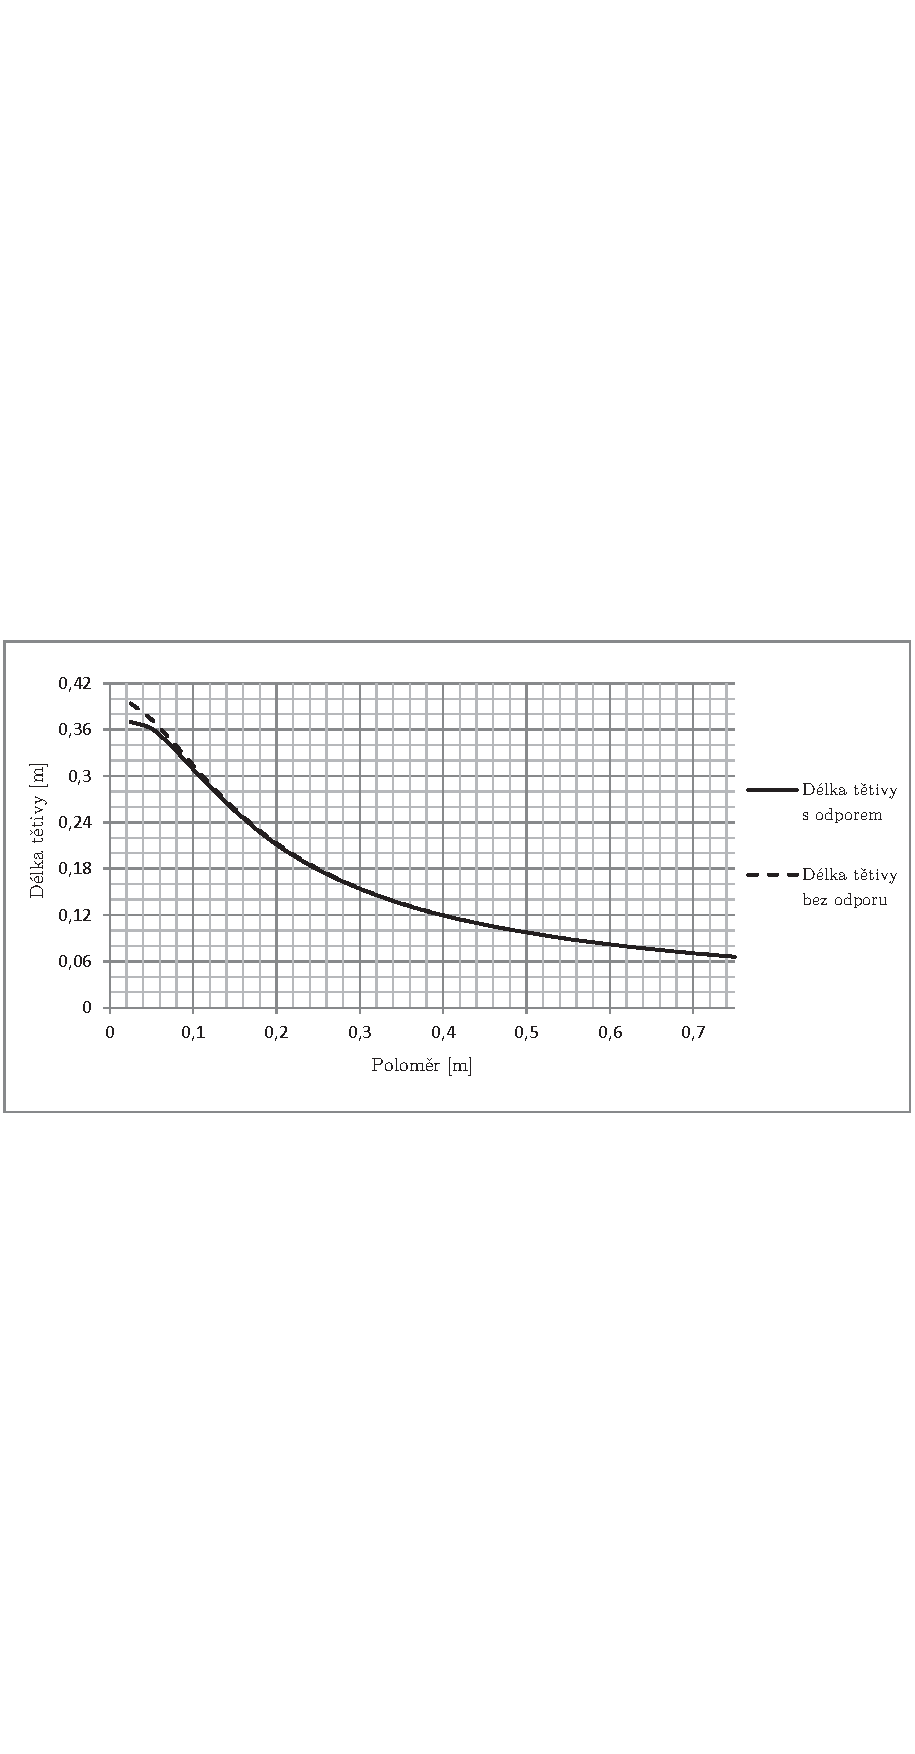
\includegraphics[]{obrazky/grafy/delkap}
		          %\input{obrazky/rotor2.ipe}
			\caption{Délka tětivy prvního prototypu trubíny. Turbína má tři listy, rychloběžnost 4, a poloměr 75~cm. Používá profil SG6043 s $c_x$ 1,303 a $c_y$ 0,017. Je zde patrný minimální rozdíl mezi výpočtem s~odporem a bez odporu.}
			\label{graf.delka1}
		    %\end{center}
		  \end{figure}
		  
	\begin{figure}[H]
				%\begin{center}
				\centering
					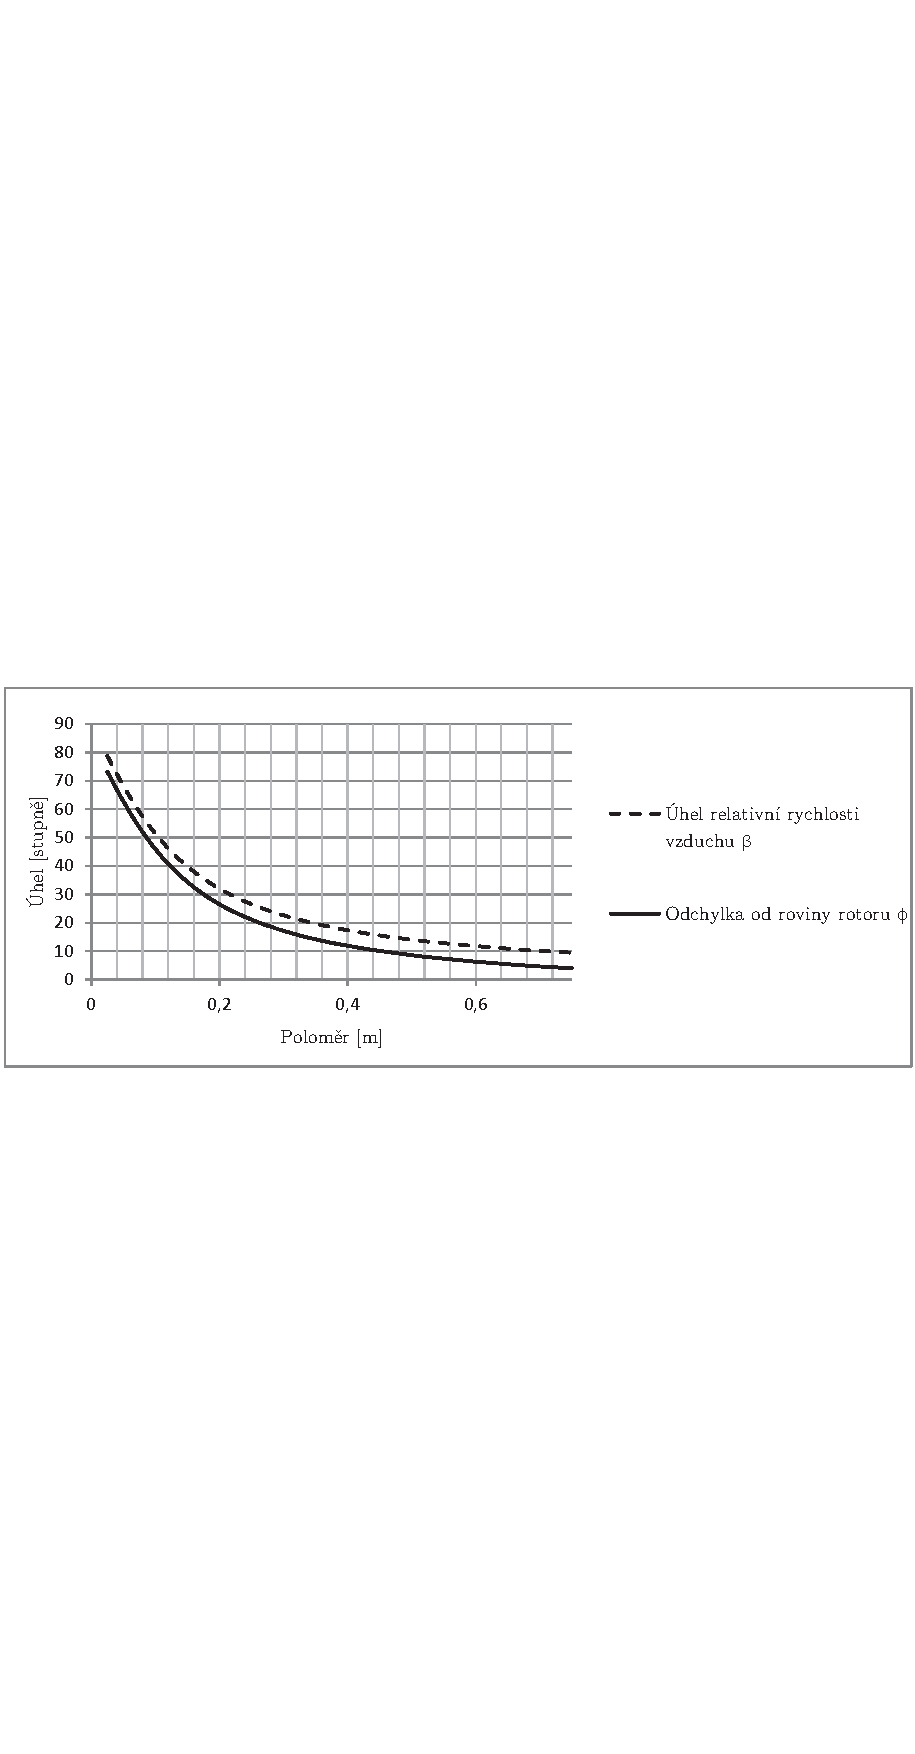
\includegraphics[]{obrazky/grafy/nabehp}
			          %\input{obrazky/rotor2.ipe}
				\caption{Graf znázorňující průběh odchylky tětivy od roviny rotoru a úhel relativní rychlosti vzduchu. Je zde uvažován ideální úhel náběhu profilu SG6043 $5,5\,^{\circ}$.}
				\label{graf.nabeh1}
			    %\end{center}
	\end{figure}
	
	
	\subsection{Rozšířený výpočet, vírová teorie}\label{kap:funkce2}
	
	Výpočet tvaru listu v předchozí kapitole má jeden nedostatek – předpokládá, že turbína proudu za rovinou rotoru neuděluje žádnou rotační složku. Avšak této vlastnosti může dosáhnout pouze ideální turbína, jejíž lopatky jsou nekonečně tenké a nevznikají na nich žádné třecí síly.
	
	Teorii uvažující vír vznikající za rotorem poprvé popsal britský aerodynamik Hermann Glauert. V této kapitole tuto teorii popisuji. Na konci této kapitoly uvádím porovnání výsledků výpočtů zjednodušené a Glauertovy teorie.
	
	Glauertova vírová teorie předpokládá, že proud vzduchu před rotorem má nulovou rotační složku (úhlová rychlost je nulová). Po průchodu rotorem bude proudu vzduchu udělena úhlová rychlost $\Omega$. Stejně jako v předchozí teorii, platí, že rychlost $v$~v rovině rotoru je aritmetickým průměrem rychlosti před rotorem $v_1$ a rychlosti za rotorem     $v_2$. Obdobně je i úhlová rychlost proudu v rovině aritmetickým průměrem rychlosti před rotorem a za ním; tedy $\frac{\Omega}{2}$\cite{Rychetnik:Motory}.
	
	Pro další úvahy je vhodné vyjádřit přírůstek úhlové rychlosti proudu vzduchu k~úhlové rychlosti rotoru $\omega$ pomocí koeficientu $h$ a poměr rychlostí před a za rotorem pomocí koeficientu~$k$.
	
	Jelikož má tento vír opačný směr otáčení než rotor, platí výraz \eqref{rov:31}\cite{Rychetnik:Motory}.
	
		\begin{eqnarray}
			\label{rov:31}
			\omega + \Omega = h\omega \nonumber \\
			\Omega = (h-1)\omega
		\end{eqnarray}
	Obdobně lze vyjádřit poměr rychlostí $v_1$ a $v_2$ \eqref{rov:32}\cite{Rychetnik:Motory}.
	\begin{eqnarray}
				\label{rov:32}
				k = \frac{v_2}{v_1} \nonumber \\
				v_2 = kv_1
	\end{eqnarray}
	Úhlovou rychlost proudu v rovině rotoru lze pomocí koeficientu vyjádřit následovně \eqref{rov:33}\cite{Rychetnik:Motory}:
	\begin{equation}
		\label{rov:33}
		\omega + \frac{\Omega}{2}=\frac{1+h}{2}\omega
	\end{equation}
	Stejně tak rychlost proudu vzduchu v rovině rotoru $v$ lze vyjádřit pomocí koeficientu $k$ - vztah \eqref{rov:34}\cite{Rychetnik:Motory}:
	\begin{equation}
			\label{rov:34}
			v =\frac{v_1 + v_2}{2}=\frac{1+k}{2}v_1
	\end{equation}
	Dalším cílem je pomocí nově definovaných rychlostí určit úhel relativní rychlosti proudu vzduchu $\beta$. Jeho určení je podobné jako ve zjednodušené teorii – vychází z obrázku \ref{obr.profilprostor}.
	Pro vyjádření úhlu $\beta$ je zapotřebí znát obvodovou rychlost prvku na rotoru ve vzdálenosti $r$ od osy otáčení \eqref{rov:35}\cite{Rychetnik:Motory}.
	\begin{equation}
		\label{rov:35}
		u =\frac{1+h}{2}\omega r
		\end{equation}
	Úhel $\beta$, který svírá směr relativní rychlosti proudu vzduchu $w$ s rovinou rotoru, lze potom vyjádřit následovně \eqref{rov:36}\cite{Rychetnik:Motory}:
	\begin{equation}
			\label{rov:36}
			\cot \beta = \frac{u}{v}=\frac{\frac{1+h}{2}\omega r}{\frac{1+k}{2}v_1}=\frac{1+h}{1+k}\lambda_r
	\end{equation}
	Velikost rychlosti $w$ je z~obrázku \ref{obr.profilprostor} rovna\eqref{rov:37}\cite{Rychetnik:Motory}:
	\begin{equation}
		\label{rov:37}
		w=\frac{v_1 (1+k)}{2\sin\beta}=\frac{\omega r(1+h)}{2\cos\beta}
	\end{equation}
	Další kroky jsou v podstatě stejné jako u zjednodušené teorie – je tedy nutné vyjádřit jednotlivé síly působící na elementy rotorového listu pomocí základní aerodynamiky vzduchového proudu a aerodynamických vlastností profilu listu. Pouze se zde dosazují výše odvozené rychlosti.
	
	Tudíž z výše uvedených vztahů lze sestavit rovnici pro axiální sílu $F_a$ - vztah \eqref{rov:38}\cite{Rychetnik:Motory}:
	\begin{equation}
		\label{rov:38}
	\mathrm{d}F_a = \mathrm{d}F_y\cos\beta+\mathrm{d}F_x\sin\beta = \frac{1}{2}\rho bw^2\; \mathrm{d}r(c_y\cos\beta + c_x\sin\beta)
	\end{equation}
	Obdobně lze také sestavit výraz pro tangenciální sílu $F_t$ \eqref{rov:39}. V~knize \cite{Rychetnik:Motory} je opět zaměněno znaménko.
	\begin{equation}
			\label{rov:39}
		\mathrm{d}F_t = \mathrm{d}F_y\sin\beta-\mathrm{d}F_x\cos\beta = \frac{1}{2}\rho bw^2\; \mathrm{d}r(c_y\sin\beta - c_x\cos\beta)
		\end{equation}
	Jelikož se zde objevují výrazy s~goniometrickými funkcemi, je výhodné převést vyjádření součinitelů vztlaku a odporu na goniometrický tvar. Celý převod vychází z obrázku \ref{obr.epsilon}.
	\begin{figure}[H]
					\centering
						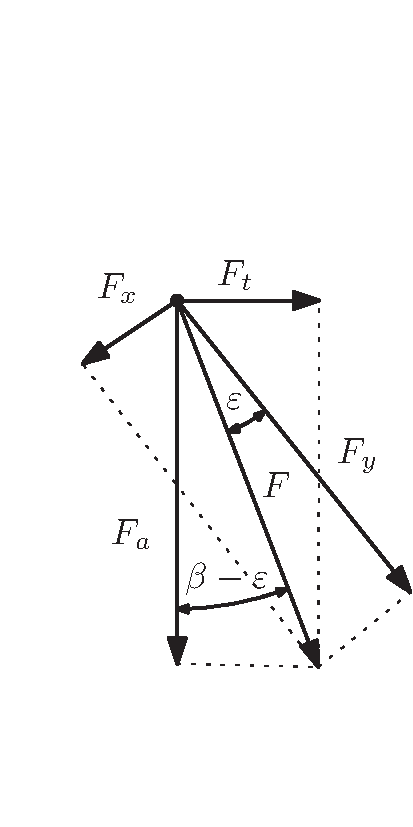
\includegraphics[]{obrazky/odvozeniepsilonp}
					\caption{Obrázek znázorňuje vyjádření sil $F_a$ a $F_t$ pomocí úhlu $\varepsilon$}
					\label{obr.epsilon}
				    %\end{center}
	\end{figure}
	Z obrázku \ref{obr.epsilon} vyplývá výraz \eqref{rov:40}\cite{Rychetnik:Motory}.
	\begin{equation}
		\label{rov:40}
		\tan \varepsilon = \frac{F_x}{F_y} = \frac{c_x}{c_y}
	\end{equation}
	Poté lze vyjádřit sílu $F_a$ následovně \eqref{rov:41}\cite{Rychetnik:Motory}:
	\begin{eqnarray}
		\label{rov:41}
		\cos \varepsilon = \frac{F_y}{F}\Rightarrow F=\frac{F_y}{\cos \varepsilon} \nonumber \\
		F_a = F\cos(\beta-\varepsilon)=\frac{F_y}{\cos\varepsilon}\cos(\beta-\varepsilon) \nonumber \\
		\mathrm{d}F_a=\frac{1}{2}\rho bw^2\;\mathrm{d}r\frac{c_y}{\cos\varepsilon}\cos(\beta - \varepsilon)
	\end{eqnarray}
	Obdobně lze vyjádřit i sílu Ft\eqref{rov:42}\cite{Rychetnik:Motory} a celkovou axiální sílu působící na všechny listy rotoru\eqref{rov:43}\cite{Rychetnik:Motory}.
	\begin{equation}
		\label{rov:42}
		\mathrm{d}F_t=\frac{1}{2}\rho bw^2\;\mathrm{d}r\frac{c_x}{\cos\varepsilon}\sin(\beta - \varepsilon)
	\end{equation}
	\begin{equation}
		\label{rov:43}
		\mathrm{d}F_{az}=\frac{1}{2}z\rho bw^2\;\mathrm{d}r\frac{c_y}{\cos\varepsilon}\cos(\beta - \varepsilon)
	\end{equation}
	Pomocí síly $F_t$ lze vyjádřit i celkový moment síly působící na všechny listy rotoru\eqref{rov:44}\cite{Rychetnik:Motory}.
	\begin{equation}
			\label{rov:44}
			\mathrm{d}M=rz\;\mathrm{d}F_t=\frac{1}{2}rz\rho bw^2\;\mathrm{d}r\frac{c_x}{\cos\varepsilon}\sin(\beta - \varepsilon)
		\end{equation}
	Axiální sílu na rotor lze stejně jako v odvození Betzovy účinnosti pomocí změny hybnosti proudu vzduchu. Proud vzduchu v~prstenci mezi poloměry $r$ a $r + \mathrm{d}r$ působí silou $\mathrm{d}F_a$ vyjádřené dle \eqref{rov:45}\cite{Rychetnik:Motory}.
	\begin{eqnarray}
		\label{rov:45}
		\mathrm{d}F_a\Delta t=m(v_1-v_2) \nonumber \\
		m=2\pi\rho r\;\mathrm{d}rv=\pi\rho r\;\mathrm{d}r(1+k)v_1 \nonumber \\
		\mathrm{d}F_a=\pi\rho r\;\mathrm{d}r(1+k)v_1\Delta v = \pi\rho r\;\mathrm{d}r(1-k^2)v_1^2
	\end{eqnarray}
	Moment síly na element rotoru mezi poloměry $r$ a $r + \mathrm{d}r$ lze také určit i ze změny momentu hybnosti proudu\eqref{rov:46}\cite{Rychetnik:Motory}. Jelikož je úhlová rychlost proudu před rotorem nulová, je změna úhlové rychlosti rovna $\Omega$.
	\begin{eqnarray}
		\label{rov:46}
		\mathrm{d}M = mru = mr^2\Omega \nonumber \\
		\mathrm{d}M=\rho\pi r^3\; \mathrm{d}r v_1(1+k)\Omega = \rho\pi r^3\; \mathrm{d}r v_1\omega(1+k)(h-1)
		\end{eqnarray}
		Další krok je podobný jako ve zjednodušené teorii – je nutné stejné, ale jinak vyjádřené, veličiny porovnat. Porovnáním axiální síly z rovnic \eqref{rov:43} a \eqref{rov:45} a dosazením relativní rychlosti proudu vzduchu $w$ z~rovnice \eqref{rov:37} dostaneme \eqref{rov:47}\cite{Rychetnik:Motory}.
		\begin{eqnarray}
			\label{rov:47}
			\frac{1}{2}\rho bzw^2\;\mathrm{d}r\frac{c_y}{\cos\varepsilon}\cos(\beta-\varepsilon)=\pi\rho r\;\mathrm{d}r(1-k^2)v_1^2 \nonumber \\
			\frac{1}{2} v_1^2\rho b \left(\frac{v_1(1+k)}{2\sin\beta}\right)^2\;\mathrm{d}r\frac{c_y}{\cos\varepsilon}\cos(\beta-\varepsilon)=\pi\rho r\; \mathrm{d}r(1-k^2)v_1^2 \nonumber \\
			c_y zb = \frac{8\pi r(1-k)\cos\varepsilon\sin^2 \beta}{\cos(\beta-\epsilon)(1+k)} \nonumber \\
			\frac{1-k}{1+k}=\frac{c_y zb \cos(\beta-\varepsilon)}{8\pi r \cos\varepsilon\sin^2\beta}
		\end{eqnarray}
		Stejnou úpravu je možné provést i s momentem síly vznikajícím na rotoru. Porovnáním rovnic \eqref{rov:44} a \eqref{rov:46} a dosazením rovnice \eqref{rov:37} dostaneme výraz \eqref{rov:48}\cite{Rychetnik:Motory}.
		\begin{eqnarray}
			\label{rov:48}
			\rho\pi r^3\;\mathrm{d}r v_1\omega(1+k)(h-1)=\frac{1}{2}rz\rho bw^2\;\mathrm{d}r\frac{c_x}{\cos \varepsilon}\sin(\beta-\varepsilon) \nonumber \\
			c_y zb = \frac{8\pi r(h-1)\cos\varepsilon\sin \beta \cos\beta}{\sin(\beta-\epsilon)(h+1)} \nonumber \\
			\frac{h-1}{h+1}=\frac{c_y zb \sin(\beta-\varepsilon)}{8\pi r \cos\varepsilon\sin\beta\cos\beta}
		\end{eqnarray}
		V knize \cite{Rychetnik:Motory} autor dává do poměru psolední řádky rovnic \eqref{rov:47} a \eqref{rov:48}. Tento postup je dle mě zbytečně složitý. Ekvivalentní výsledek, s jednodušší úpravou, lze získat porovnáním  vyjádření $c_yzb$ \eqref{rov:49}.
		\begin{eqnarray}
			\label{rov:49}
			\frac{8\pi r(1-k)\cos\varepsilon\sin^2 \beta}{\cos(\beta-\epsilon)(1+k)}=\frac{8\pi r(h-1)\cos\varepsilon\sin \beta \cos\beta}{\sin(\beta-\epsilon)(h+1)} \nonumber \\
			(1-k)(h+1)\sin(\beta-\varepsilon)\sin\beta=(h-1)(k+1)\cos\beta\cos(\beta-\varepsilon) \nonumber \\
			\frac{(1-k)(h+1)}{(h-1)(k+1)}=\frac{\cos\beta\cos(\beta-\epsilon)}{\sin\beta\sin(\beta-\epsilon)}=\cot(\beta-\varepsilon)\cot\beta
		\end{eqnarray}
		Zde je patrné, proč byla úprava poměru součinitelů $c_x$ a $c_y$ na $\tan\varepsilon$ (výraz \eqref{rov:40}) provedena – výrazně zjednodušila výsledný tvar.
		
		Ačkoliv to není přímo patrné, vyplývá z rovnice \eqref{rov:49} výpočet rotorového listu. Výpočet je složitější než v prvním případě. Jsou zde 2 proměnné (koeficienty $h$ a $k$), které jsou na sobě cyklicky závislé – jeden vyplývá z druhého. Tato soustava jde řešit pouze iteračně. Přesný postup výpočtu popisuji dále v kapitole \ref{postup}. Na grafu \ref{graf.glauert1} je zobrazeno porovnání délek tětiv zjednodušeného a Gluertova výpočtu. Tento graf je sestrojen pro turbínu stejných parametrů, na jaké byl konstruován první prototyp.
		
		Křivka grafu \ref{graf.glauert1}, která znázorňuje tvar listu, je velmi podobná vyobrazení ideálního rotoru na obrázku 5.2-5 v knize \cite{Crome:Technika} (strana 44). Je také vidět, že výpočet podle Glauerta dává výrazně jiné hodnoty v oblasti blízko osy otáčení než základní teorie.
		Porovnání úhlů náběhu mezi základním výpočtem a výpočtem podle Glauerta je zobrazeno na grafu \ref{graf.glauert2}. Hodnoty se výrazněji liší pouze blízko u osy otáčení (stejně jako v případě tětivy).
		
		
		\begin{figure}[h]
						%\begin{center}
						\centering
							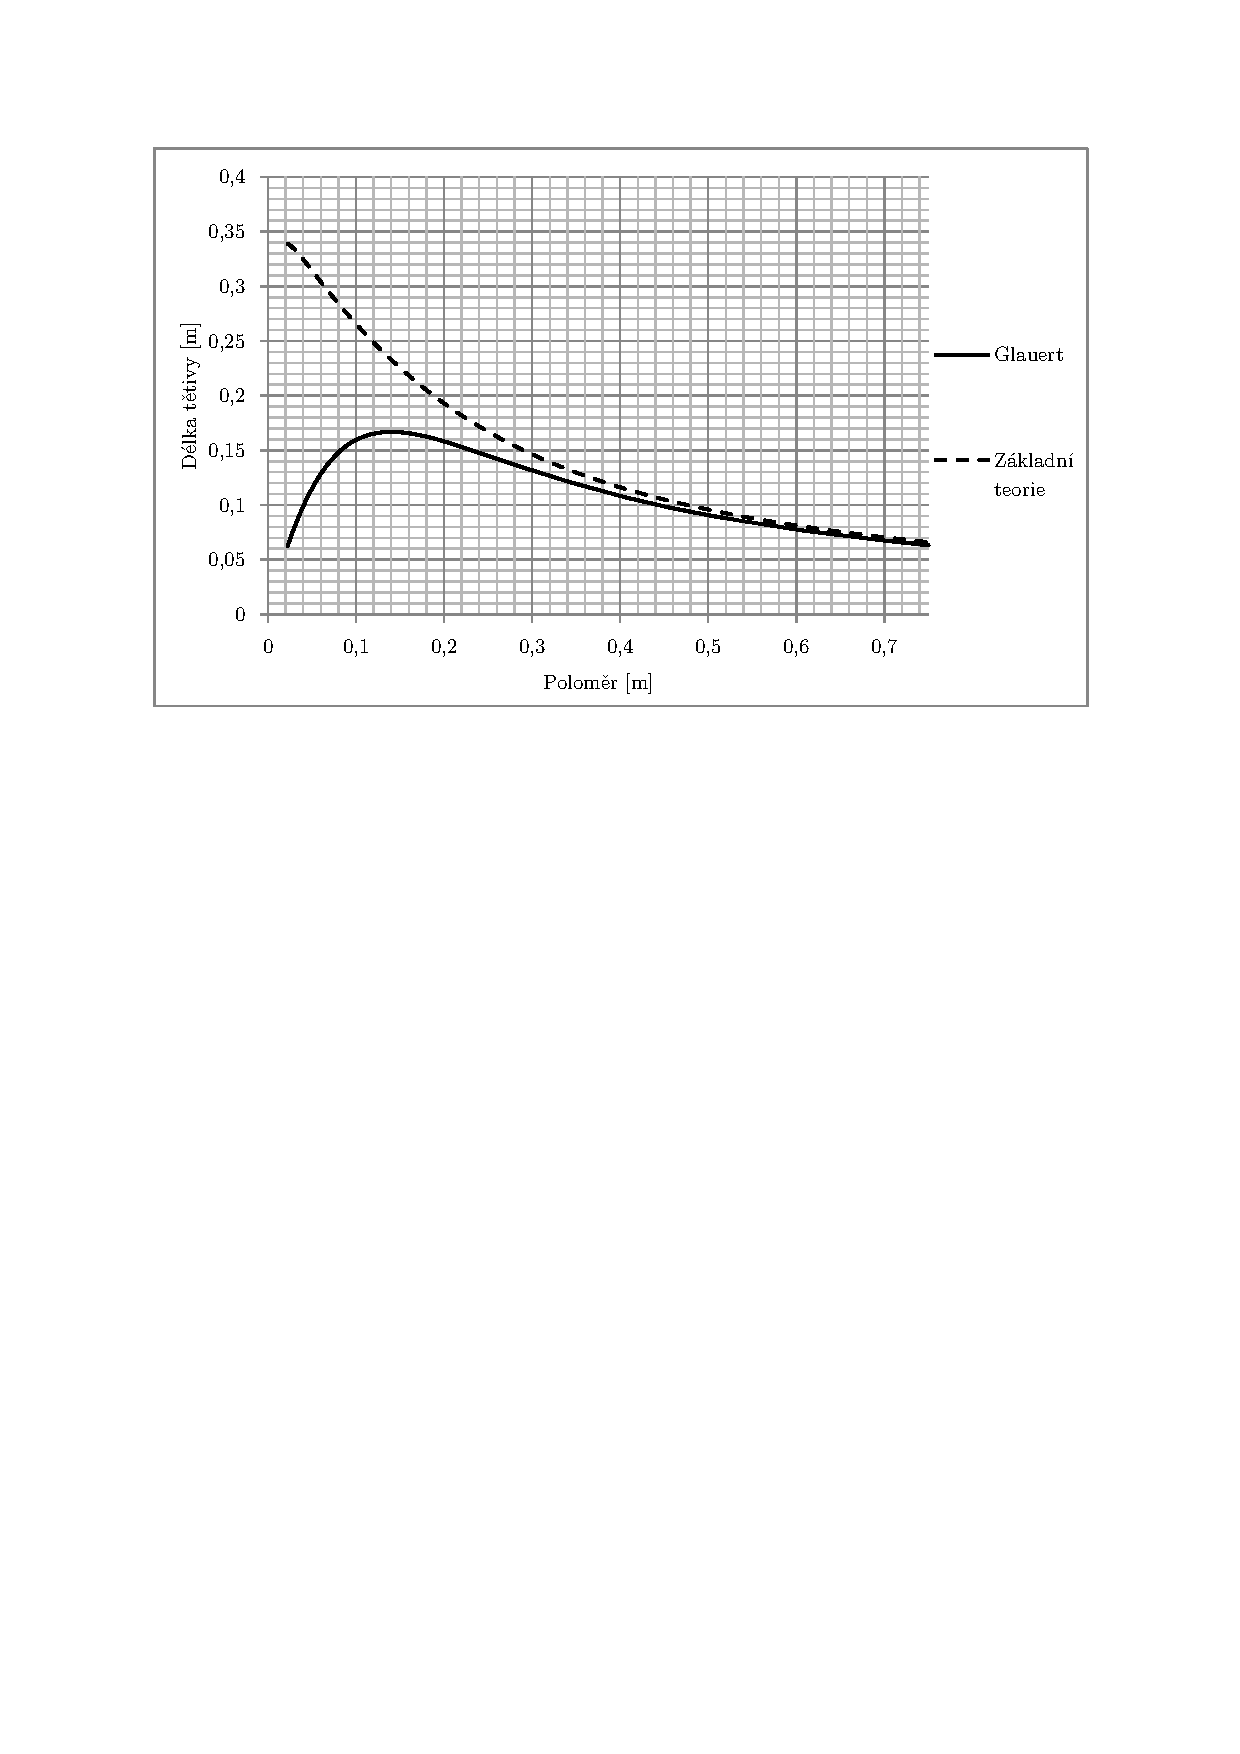
\includegraphics[]{obrazky/grafy/glauert1}
					          %\input{obrazky/rotor2.ipe}
						\caption{Graf porovánává délky tětiv pro zjednodušenou teorii a pro teorii podle Glauerta. List je počítán pro stejné parametry jako v grafu \ref{graf.delka1}}
						\label{graf.glauert1}
					    %\end{center}
		\end{figure}
		\begin{figure}[h]
								%\begin{center}
								\centering
									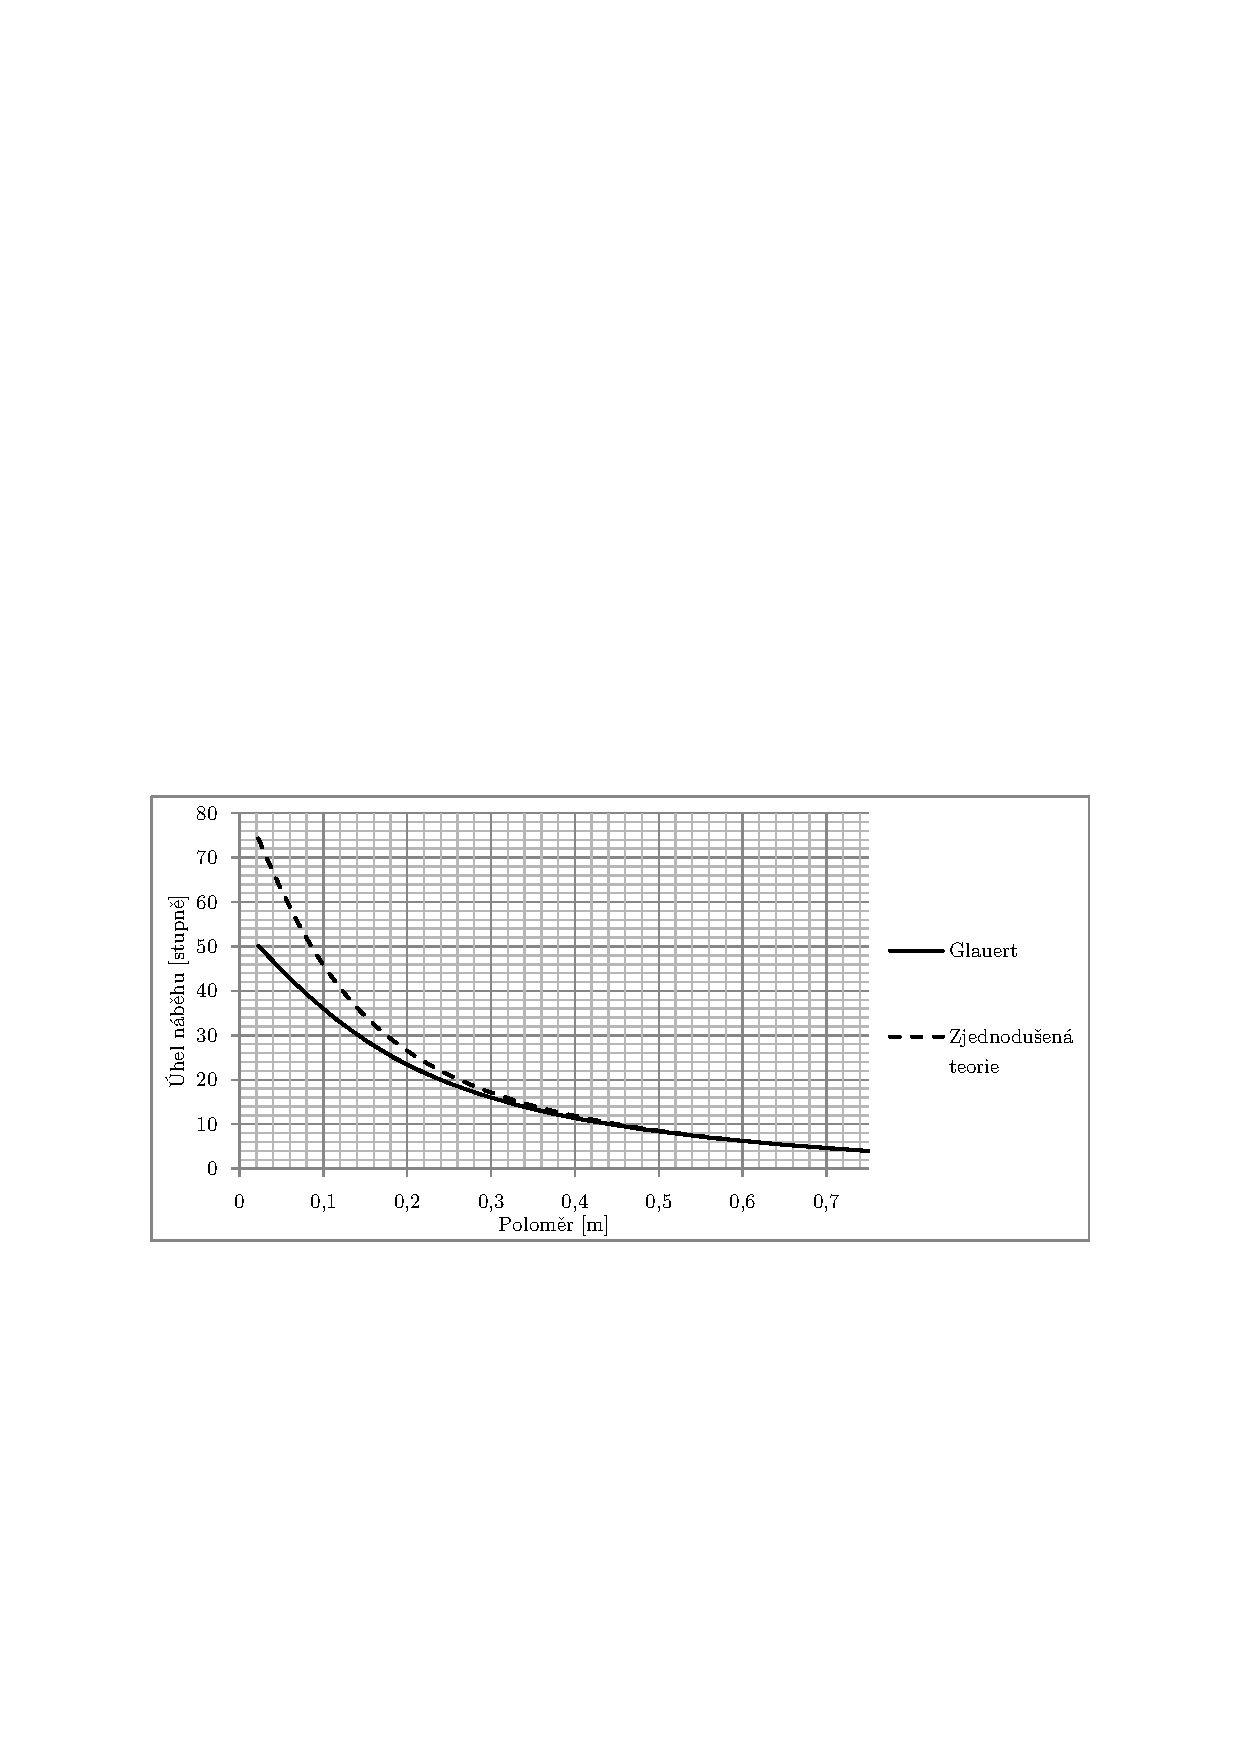
\includegraphics[]{obrazky/grafy/glauert2}
							          %\input{obrazky/rotor2.ipe}
								\caption{Porovnání úhlu náběhu pro zjednodušenou teorii a výpočet podle Glauerta. List je počítán pro stejné parametry jako v grafu \ref{graf.delka1}}
								\label{graf.glauert2}
							    %\end{center}
				\end{figure}